\chapter{Diseño e implementación} % Main chapter title

Este capítulo presenta la arquitectura del sistema embebido, la estructura de los componentes de software principales, las consideraciones en la selección de componentes electrónicos y los diseños del PCB y del gabinete del sistema.

\label{Chapter3} % Change X to a consecutive number; for referencing this chapter elsewhere, use \ref{ChapterX}

\definecolor{mygreen}{rgb}{0,0.6,0}
\definecolor{mygray}{rgb}{0.5,0.5,0.5}
\definecolor{mymauve}{rgb}{0.58,0,0.82}

%%%%%%%%%%%%%%%%%%%%%%%%%%%%%%%%%%%%%%%%%%%%%%%%%%%%%%%%%%%%%%%%%%%%%%%%%%%%%
% parámetros para configurar el formato del código en los entornos lstlisting
%%%%%%%%%%%%%%%%%%%%%%%%%%%%%%%%%%%%%%%%%%%%%%%%%%%%%%%%%%%%%%%%%%%%%%%%%%%%%
\lstset{ %
  backgroundcolor=\color{white},   % choose the background color; you must add \usepackage{color} or \usepackage{xcolor}
  basicstyle=\footnotesize,        % the size of the fonts that are used for the code
  breakatwhitespace=false,         % sets if automatic breaks should only happen at whitespace
  breaklines=true,                 % sets automatic line breaking
  captionpos=b,                    % sets the caption-position to bottom
  commentstyle=\color{mygreen},    % comment style
  deletekeywords={...},            % if you want to delete keywords from the given language
  %escapeinside={\%*}{*)},          % if you want to add LaTeX within your code
  %extendedchars=true,              % lets you use non-ASCII characters; for 8-bits encodings only, does not work with UTF-8
  %frame=single,	                % adds a frame around the code
  keepspaces=true,                 % keeps spaces in text, useful for keeping indentation of code (possibly needs columns=flexible)
  keywordstyle=\color{blue},       % keyword style
  language=[ANSI]C,                % the language of the code
  %otherkeywords={*,...},           % if you want to add more keywords to the set
  numbers=left,                    % where to put the line-numbers; possible values are (none, left, right)
  numbersep=5pt,                   % how far the line-numbers are from the code
  numberstyle=\tiny\color{mygray}, % the style that is used for the line-numbers
  rulecolor=\color{black},         % if not set, the frame-color may be changed on line-breaks within not-black text (e.g. comments (green here))
  showspaces=false,                % show spaces everywhere adding particular underscores; it overrides 'showstringspaces'
  showstringspaces=false,          % underline spaces within strings only
  showtabs=false,                  % show tabs within strings adding particular underscores
  stepnumber=1,                    % the step between two line-numbers. If it's 1, each line will be numbered
  stringstyle=\color{mymauve},     % string literal style
  tabsize=2,	                   % sets default tabsize to 2 spaces
  title=\lstname,                  % show the filename of files included with \lstinputlisting; also try caption instead of title
  morecomment=[s]{/*}{*/}
}


%----------------------------------------------------------------------------------------
%	SECTION 1
%----------------------------------------------------------------------------------------
\section{Arquitectura del sistema embebido}

En la figura \ref{fig:arquitectura_sistema} se muestra un diagrama de bloques con la arquitectura del sistema SCI-CAN y sus interacciones. El recuadro marcado como controlador corresponde a lo desarrollado en este trabajo. En los recuadros externos están los dispositivos con los que este sistema debe interactuar: PLCs, servomotores SN-17 y PC.

La interacción con los PLC se realiza a través de señales discretas que necesitan estar acondicionadas según especificaciones \citep{plan_trabajo}. Con los servomotores la comunicación se realiza a través de un bus CAN. Por otro lado, la interacción con una PC se consigue utilizando un conversor USB - UART.

\begin{figure}[h!]
	\centering
	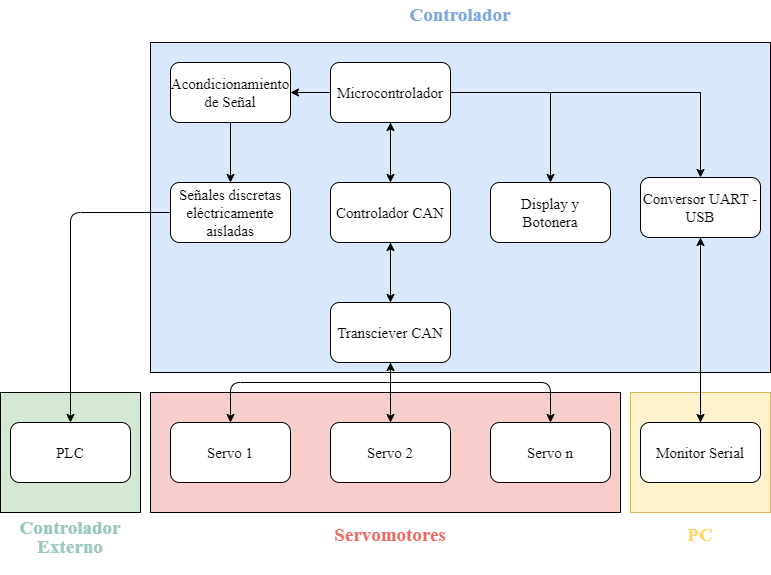
\includegraphics[scale=.5]{./Figures/Arquitectura_SE.png}
	\caption{Arquitectura del sistema.}
	\label{fig:arquitectura_sistema}
\end{figure}

Las interacciones internas del sistema incluyen:
\begin{itemize}
	\item Periférico controlador y \textit{transceiver} CAN.
	\item Señales discretas eléctricamente aisladas de la alimentación del sistema.
	\item Display LCD con protocolo I2C.
	\item Teclado matricial mediante IOs.
	\item Puerto USB empleando protocolo UART y un conversor USB - UART.
\end{itemize}

El usuario puede interactuar con el sistema de las siguientes formas:
\begin{itemize}
	\item Display: visualización de la información de los servomotores.
	\item Teclado: navegación a través de los menúes del display.
	\item PC: monitor serial para envío de configuraciones.
\end{itemize}

\newpage

\section{Selección de componentes}
\label{seccion_seleccion_componentes}

Previo al desarrollo del hardware y del software se determinaron los componentes a utilizar en el diseño. 

En general, se buscó que los componentes tengan las siguientes características:
\begin{itemize}
	\item Disponibilidad en el mercado.
	\item Facilidad para ensamble manual.
	\item Conocimiento previo sobre su uso.
	\item Bajo costo.
\end{itemize}

La falta de disponibilidad de los componentes se convirtió en uno de los mayores riesgos durante el desarrollo del proyecto, debido al desabastecimiento de electrónica presente en el transcurso de la pandemia Covid-19.

Los componentes electrónicos seleccionados fueron:

\begin{itemize}
	\item Microcontrolador ATSAMC21G18A \citep{web_ATSAMC21G18A}: es el mismo modelo empleado en los sistemas SN-17, posee un controlador CAN integrado.
	\item Transceiver CAN LTC2875IS8 \citep{web_transciever_CAN}: también utilizado en el sistema SN-17.
	\item Regulador de tensión LM2575 \citep{web_LM2575}: cumple con los requerimientos de alimentación y de temperatura del sistema.
	\item Interfaz USB - UART CY7C64225 \citep{web_interfaz_USB_UART}: posee drivers USB para interactuar con Windows.
	\item Optoacopladores LTV-846S \citep{web_optoacopladores_LTV}: cumplen con el requerimiento de aislación eléctrica de 1 KV, cuentan con 4 canales y poseen el menor \textit{footprint} entre las opciones disponibles.
\end{itemize}

Una vez seleccionados todos los componentes principales del sistema se estudiaron sus hojas de datos y se seleccionaron los componentes periféricos indicados en ellas. Con esta información se completó el listado de componentes del PCB.

Los componentes de interfaz elegidos fueron:
\begin{itemize}
	\item Display LCD de veinte caracteres y cuatro líneas con controlador HD44780 e interfaz de programación I2C. 
	\item Teclado matricial de cuatro filas por cuatro columnas del fabricante Adafruit \citep{web_adafruit} (figura \ref{fig:keypad}). Este es mecánicamente robusto para poder ser utilizado en un ambiente industrial. 
\end{itemize}

\begin{figure}[htbp]
	\centering
	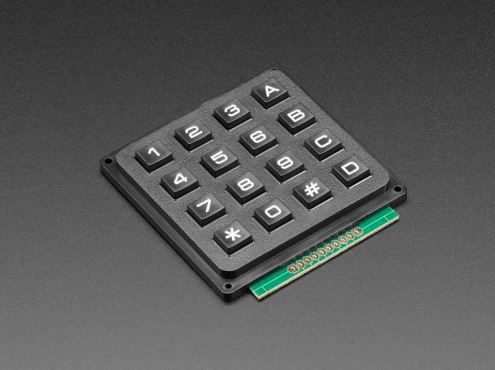
\includegraphics[scale=.8]{./Figures/keypad.JPG}
	\caption{Teclado matricial Adafruit 4x4.}
	\label{fig:keypad}
\end{figure}



\section{Comunicación CAN}
\label{comunicacion_can}

La implementación de una red CAN requiere consideraciones de diseño relacionadas con el \textit{bitrate} y los tiempos de bit con los cuales trabaja el protocolo para la lectura y envío de información. Como se explicó en la sección \ref{caracteristicas_can}, estas variables están relacionadas con la longitud del bus y con el ruido eléctrico al que está expuesto. En la tabla \ref{tab:bit_times} se presentan los tiempos de bit recomendados para implementaciones de CANopen \citep{UnderstandingCAN}. Del listado se seleccionó la fila para un bus de 250 m, que recomienda un \textit{bitrate} de 250 kb/s. Estos parámetros se configuraron en el periférico CAN del microcontrolador.

\newpage

\begin{table}[h!]
	\centering
	\caption[Tiempos de bit recomendados para CANopen.]{Tiempos de bit recomendados para CANopen.}
	\begin{tabular}{c c c c c c}    
		\toprule
		\textbf{\textit{Bitrate}} & \textbf{Largo bus} & \textbf{Tiempo bit} & \textbf{\textit{Time quanta}} & \textbf{\textit{N quanta}} & \textbf{\textit{Sample}} \\
		\midrule
		1 Mb/s 		& 25 m 	& 1 $\mu$s		& 125 ns & 8 	& 6 \\
		800 kb/s 	& 50 m 	& 1,25 $\mu$s	& 125 ns & 10 	& 8 \\
		500 kb/s 	& 100 m & 2 $\mu$s		& 125 ns & 16 	& 14 \\
		250 kb/s 	& 250 m & 4 $\mu$s		& 250 ns & 16 	& 14 \\
		125 kb/s 	& 500 m & 8 $\mu$s		& 500 ns & 16 	& 14 \\
		50 kb/s 	& 1000 m & 20 $\mu$s	& 1,25 $\mu$s & 16 	& 14 \\
		20 kb/s 	& 2500 m & 50 $\mu$s	& 3,125 $\mu$s & 16 	& 14 \\
		10 kb/s 	& 5000 m & 100 $\mu$s	& 6,25 $\mu$s & 16 	& 14 \\
		\bottomrule
		\hline
	\end{tabular}
	\label{tab:bit_times}
\end{table}

La estructura empleada para la codificación de la información dentro de los mensajes CAN se muestra en la figura \ref{fig:estructura_mensajes}. Se utilizaron tanto el campo de identificador estándar de 11 bits, como los bytes de data para indicar el tipo de mensaje y la manera en que debe ser procesado.

\begin{figure}[h!]
	\centering
	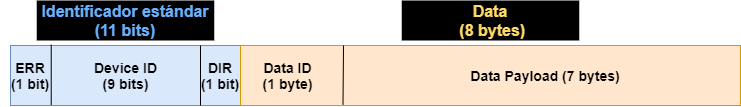
\includegraphics[width=1\linewidth ,height=0.12\textheight]{./Figures/estructura_mensaje.png}
	\caption{Estructura de mensajes CAN}
	\label{fig:estructura_mensajes}
\end{figure}

Dentro del campo identificador se codificó la siguiente información:
\begin{itemize}
	\item Bit 1: identificador de error.
	\item Bits 2 a 10: \textit{device ID}. Detalla el identificador único y fijo del dispositivo en la red.
	\item Bit 11: dirección. Define si un mensaje es envíado por un dispositivo controlador de red (SCI-CAN) o un dispositivo periférico (SN-17).
\end{itemize}

Se estableció el primer bit del mensaje como identificación de errores para que  estos tengan la mayor prioridad en el proceso de arbitraje de la red CAN. Además, los mensajes que tienen este bit encendido no son filtrados por ningún dispositivo de la red.

En los bits que corresponden al \textit{device ID} también se especifican identificadores comunes para mensajes del tipo \textit{broadcast}. Estos permiten la transmisión de información a todos los nodos de la red.



El campo de data tiene una longitud total de 8 bytes. Este contiene la siguiente información:
\begin{itemize}
	\item Byte 1: \textit{data ID}. Identifica el tipo de información del mensaje según la tabla \ref{tab:tipos_mensajes_CAN}.
	\item Bytes 2 a 8: \textit{data payload}. Contiene la información codificada según el \textit{data ID}.
\end{itemize}

La tabla \ref{tab:tipos_mensajes_CAN} presenta todos los \textit{data ID} implementados en el sistema. Para cada uno de estos tipos de mensaje la información se codifica de una forma diferente.

\begin{table}[h]
	\centering
	\caption[Operaciones SN-17]{Funciones de SN-17}
	\begin{tabular}{c c c}    
		\toprule
		\textbf{\textit{Data ID}} 	& \textbf{Tipo}  & \textbf{Descripción}\\
		\midrule
		Tipo de instrucción & Instrucción 	& Define la instrucción\\		
		Límite de torque 	& Instrucción	& Torque máximo de instrucción \\
		Modo de control		& Instrucción 	& Posición, velocidad, torque \\
		\textit{Set point}	& Instrucción 	& Valor de lazo de control \\
		\textit{Threshold}	& Instrucción 	& Valor de error admisible \\
		\textit{Hold time}	& Instrucción 	& Tiempo de cumplimiento \\
		\textit{Timeout}	& Instrucción 	& Tiempo de no cumplimiento \\
		Guardar posición	& Configuración & Guarda posición actual \\
		Calibrar posición	& Configuración & Guarda posición manual \\
		Constantes PID		& Configuración & Constantes lazo de control \\	
		Entradas y salidas	& Configuración & Funcionamiento de las IO \\
		\textit{Homing}		& Configuración & Establece rutina de cerado \\	
		Calibración			& Comando		& Inicia la rutina de calibración \\
		Activar motor		& Comando		& Enciende/apaga el motor \\		
		\textit{Go Home}	& Comando		& Inicia la rutina de cerado \\		
		Mover motor			& Comando		& Rota un ángulo específico\\
		Rotar motor			& Comando		& Gira a velocidad específica \\
		Torquear motor		& Comando		& Gira a torque específico \\
		Límite torque manual& Comando		& Limita el torque de comandos \\
		Activar salidas		& Comando		& Enciende/apaga salidas \\	
		Consultar motor		& Comando		& Consulta información del motor \\
		Programa manual		& Comando		& Corre un programa en modo maual \\
		Instrucción actual	& Supervisión	& Instrucción ejecutada del motor \\
		Encoder				& Supervisión	& Posición de encoder del motor \\
		Error				& Supervisión	& Tipo de error del motor \\
		Cambio de modo		& General		& Programación o operación \\
		\textit{Device ID}	& General		& Consulta de IDs de red \\
		\bottomrule
		\hline
	\end{tabular}
	\label{tab:tipos_mensajes_CAN}
\end{table}

\newpage

Los tipos de mensajes implementados se dividen en:
\begin{itemize}
	\item Instrucción: identifican los comandos en la secuencia de un programa en los sistemas SN-17 durante su operación. Son de lectura y escritura.
	\item Configuración: establecen los parámetros operativos de los sistemas SN-17. Son de lectura y escritura.
	\item Comando: indican a un sistema SN-17 una acción manual a realizar. Son de solo escritura.
	\item Supervisión: indican al SCI-CAN el estado de un SN-17. Son de solo lectura.
	\item General: son mensajes del tipo \textit{broadcast} para el control de la red. Son de lectura y escritura.
\end{itemize}

Los mensajes del tipo instrucción codifican un número según el \textit{data ID} que se utilice e identifican su posición en la secuencia del programa del sistema SN-17.

Los mensajes de configuración agregan información complementaria para indicar los parámetros modificables. Por ejemplo, en el caso de una constante PID, se indica en forma codificada cual es la constante y su valor. 

\section{Desarrollo de software}
\label{desarrollo_software}

\subsection{Arquitectura de Software}

El desarrollo del software se realizó sobre una placa de evaluación del microcontrolador seleccionado \citep{web_dev_board}. Esto permitió hacer pruebas del sistema previo al diseño del circuito y facilitó el proceso de implementación.

El software del sistema se diagramó siguiendo una estructura en capas. En la figura \ref{fig:arq_software} se muestra un esquema de la arquitectura implementada. Como se puede observar, las capas intermedias interactúan con la capa superior de aplicación mediante el uso de servicios públicos que cada uno de los manejadores ofrece. Las capas inferiores (Key, LCD I2C handler, buffer circular) no son visibles por la capa de aplicación, pero ofrecen funcionalidades para las capas intermedias. 

\begin{figure}[htbp]
	\centering
	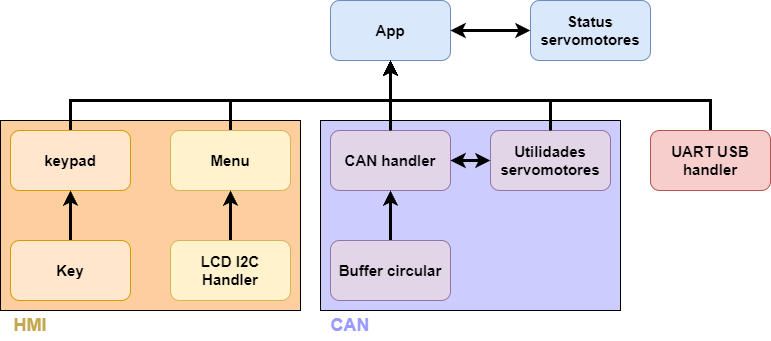
\includegraphics[scale=.5]{./Figures/arquitectura_software.png}
	\caption{Arquitectura de software}
	\label{fig:arq_software}
\end{figure}

La capa superior contiene a la aplicación que opera, en un mismo nivel, con una sección del código que almacena el estado de los distintos servomotores. En esta capa de software se coordina el funcionamiento e interacción de las capas intermedias.

El recuadro marcado como HMI (\textit{Human Machine Interface}) se relaciona con la sección del programa encargada de proveer la interfaz de usuario. Maneja las acciones del teclado matricial y la información que se visualiza en el display.

La sección CAN se relaciona con las configuraciones del periférico controlador del protocolo, las funciones para codificar los mensajes, el envío y recepción de mensajes y los servicios ofrecidos por los servomotores.

El manejador de UART-USB es el encargado de las interacciones con una PC. Realiza la codificación de información de los mensajes y procesa los datos recibidos por el puerto USB. 

En las subsecciones siguientes se explica el desarrollo de estos componentes principales de software.

\subsection{Driver CAN}

Para la implementación del módulo CAN handler de la figura \ref{fig:arq_software} se utilizó el periférico de este protocolo de comunicación en el microcontrolador seleccionado. Se realizó su configuración mediante la herramienta de desarrollo \textit{Microchip Studio} provista por el fabricante \citep{web_microchip_studio}, a través de la cual se seleccionaron:
\begin{itemize}
	\item Los tiempos de bit y la tasa de transmisión de 250 kb/s, según la tabla \ref{tab:bit_times}.
	\item El uso del identificador estándar.
	\item El funcionamiento de los filtros.
	\item La opción de reenvío de mensaje en caso de colisiones.
\end{itemize}

El driver implementado opera por interrupción, con funciones de \textit{callback} llamadas cuando se recibe un mensaje o termina una transmisión. El software de este módulo resultó de una adaptación del código de ejemplo de operación del periférico CAN provisto por el fabricante.

En la figura \ref{fig:can_handler} se observa el flujo de programa implementado para el manejo de la recepción de los mensajes CAN.

\begin{figure}[htbp]
	\centering
	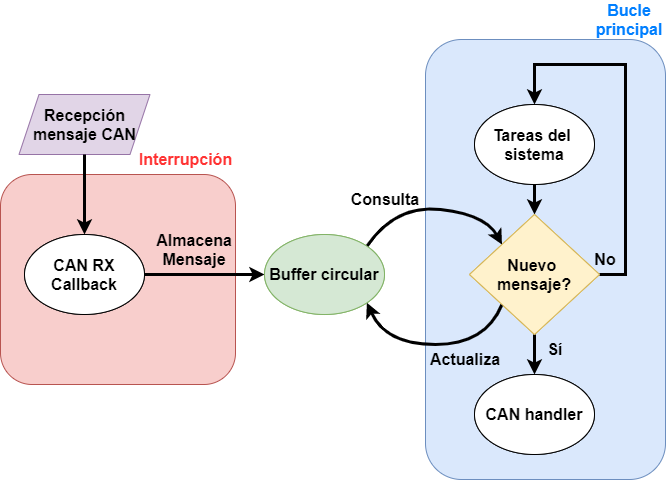
\includegraphics[scale=.5]{./Figures/Can_handler.png}
	\caption{Flujo de recepción de mensajes CAN.}
	\label{fig:can_handler}
\end{figure}

En la recepción de mensajes se empleó un módulo de software de \textit{buffer} circular \citep{tpf_gabriel}. La operación de recepción de mensajes CAN se hace en un estado de interrupción. Para evitar el procesamiento del mensaje en este estado se utiliza el algorítmo de \textit{buffer} circular, que almacena el mensaje en tiempo de interrupción sin procesarlo y señaliza esta condición. Estos mensajes son luego tratados dentro del bucle principal del programa. Este funcionamiento permite una operatoria ordenada y evita la pérdida de información en caso de que nuevos mensajes lleguen al bus sin que los anteriores hayan sido procesados.

Para la interpretación de los mensajes se construyó el módulo de software marcado como "utilidades servomotores" en la figura \ref{fig:arq_software}. Dentro de este se implementaron distintas funciones locales que decodifican el identificador y la data según el tipo de mensaje. Con el identificador CAN se determina si el mensaje recibido indica un error (primer bit) y si está dirigido a un SN-17 o al SCI-CAN (último bit de dirección). Con respecto a la información del tipo, como se explicó en la sección \ref{comunicacion_can}, se encuentra codificada en el primer byte de data del mensaje CAN. Esta información es discriminada por el algorítmo y, utilizando una estructura \textit{switch-case}, se selecciona la función decodificadora correspondiente.


\subsection{Interfaz HMI}

La interfaz HMI involucra la interacción del software del sistema con el teclado y con el display LCD. Su implementación implicó el desarrollo de los drivers de I2C para trabajar con la pantalla y manejadores para el teclado. También, se desarrolló un \textit{middleware} para controlar un sistema de menúes, así como la interacción entre ambos drivers. A su vez, este \textit{middleware} ofrece funcionalidades a la capa superior de aplicación.

La capa inferior del display se compone del driver I2C obtenido del fabricante del microcontrolador y una serie de servicios para mostrar información que son llamados por las capas superiores. Los servicios fueron modelados siguiendo ejemplos de código libre de implementaciones para Arduino \citep{web_repo_display_i2c}.

El driver del teclado sigue una arquitectura similar \citep{web_repo_keypad}. Se utilizaron como ejemplo implementaciones libres de Arduino \citep{web_repo_keypad}. Esta capa ofrece servicios a las superiores para reconocer las teclas que fueron oprimidas.

Sobre estos manejadores se desarrolló un software que utiliza a ambos para generar el sistema de menúes y controlar la interacción con un usuario. Mediante el uso del teclado se puede navegar a través de una lista de opciones que se muestran en el display y se permite visualizar y configurar los parámetros de los motores conectados. 

En la figura \ref{fig:menu} se muestra un ejemplo de cómo se presentan las opciones en el display. La flecha presente a la izquierda de la imagen es la que le permite al usuario ubicarse a medida que navega por los menúes mediante la utilización del teclado.

\begin{figure}[htbp]
	\centering
	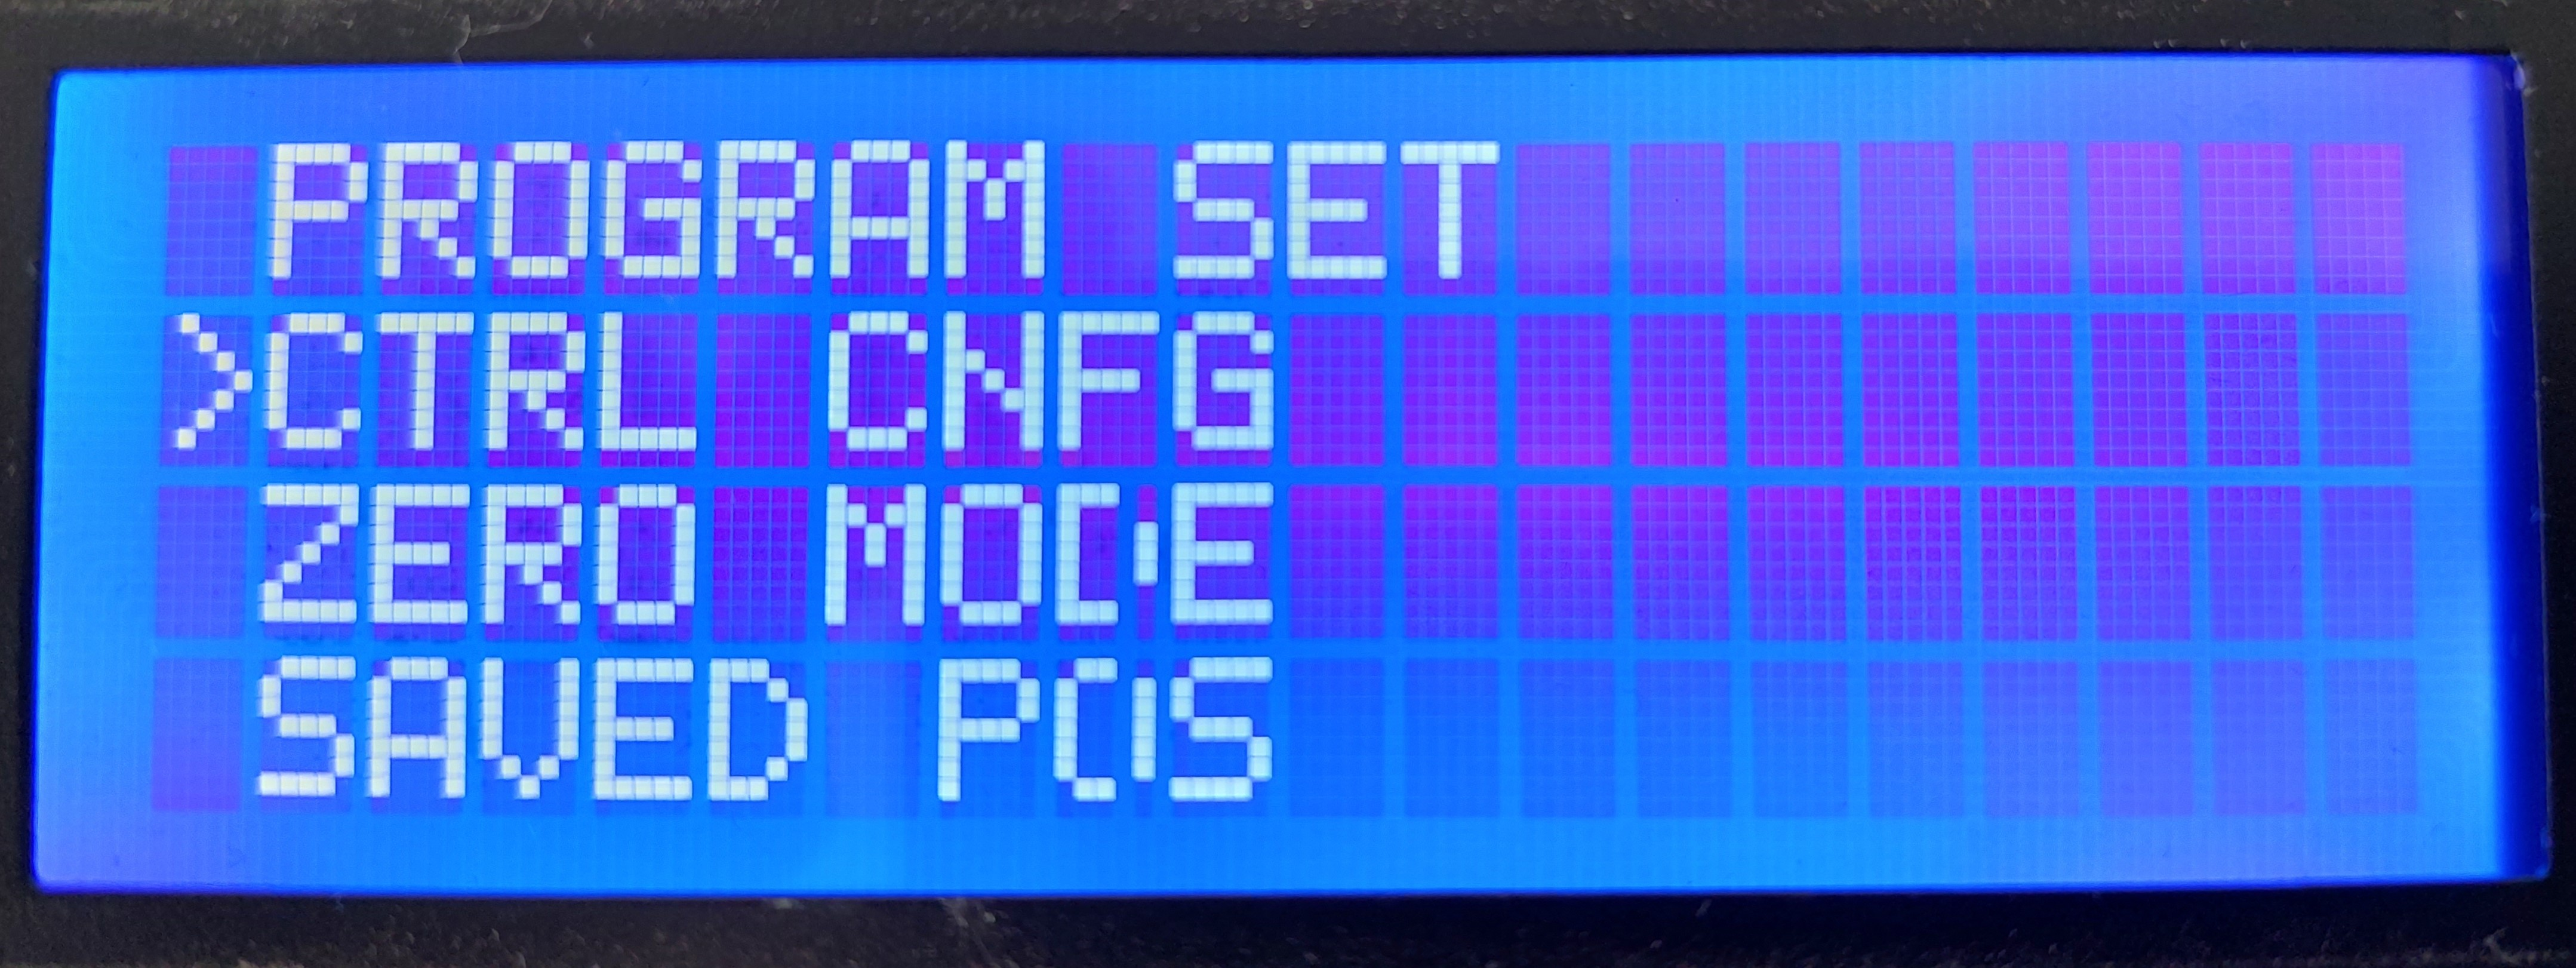
\includegraphics[scale=.08]{./Figures/display_menu.jpg}
	\caption{Ejemplo de opciones de menú}
	\label{fig:menu}
\end{figure}

Se planteó que el menú cuente con dos pantallas diferentes según el estado en el que esté el sistema: monitoreo o programación. En el estado de monitoreo, se muestra una primera pantalla donde puede observarse el programa e instrucción que cada motor conectado está ejecutando en ese momento. A su vez puede navegarse para consultar la configuración, pero no puede ser modificada.

En el estado de programación, la configuración de los distintos motores es accesible para ser modificada y se muestran los distintos comandos manuales que pueden ejecutarse para cada motor. Al pasar del estado de monitoreo al de programación, la central envía un mensaje de \textit{broadcast} usando un ID prioritario a la red al que cada motor responde con su ID particular.

El software de menúes le indica a la capa superior de aplicación la acción solicitada por el usuario y es esta capa la que interactúa con los otros drivers, como se explicó en la sección \ref{desarrollo_software}.

\subsection{Interfaz UART-USB}

La interfaz UART-USB involucró el desarrollo de un manejador de UART desde el microcontrolador. La configuración de la comunicación se realizó con herramientas provistas por el fabricante. El software opera por interrupciones de hardware que llaman a funciones de \textit{callback} al completar una transmisión o recepción de un mensaje.

Los mensajes UART son adaptados a señales USB mediante el circuito integrado CY7C64225 \citep{web_interfaz_USB_UART}. Esto permite la conexión del dispositivo con un monitor serial en una PC.

Sobre este manejador UART se construyó una herramienta de reporte que se ejecuta en la capa de aplicación y envía las acciones seleccionadas por el menú a través de USB. Esto permite confirmar que la información seleccionada es la correcta y facilita la detección de errores.

La interfaz de PC permite también configurar las acciones de los motores. La configuración una vez que llega al SCI-CAN es transformada en comandos CAN y enviada al nodo correspondiente.

\section{Modificaciones firmware SN-17}

Para que el sistema SCI-CAN pudiera comunicarse con las plaquetas SN-17 ya instaladas, se debió trabajar y actualizar su firmware. Estos cambios tuvieron 3 objetivos principales:
\begin{itemize}
	\item Incorporar los drivers de CAN y la estructura de mensajes planteada.
	\item Generar que las configuraciones y programas sean variables modificables.
	\item Lograr el almacenamiento de las configuraciones en memoria no volátil.
\end{itemize}

La implementación de CAN utilizó los mismos módulos de software desarrollados para el SCI-CAN sin modificaciones. Esto fue posible debido a que ambos sistemas utilizan el mismo microcontrolador. Siguiendo la estructura de CAN de la figura \ref{fig:arq_software}, los módulos de CAN handler y buffer circular se mantuvieron idénticos para ambos sistemas.

En la implementación del módulo de utilidades de servomotores se buscó también que ambos sistemas compartan el mismo software. Para ello, se planteó el uso de sentencias condicionales que determinen si un mensaje está dirigido a un sistema SCI-CAN o a un SN-17. A partir de esto se decide la acción a realizar en la capa de aplicación según la información del mensaje.

Para lograr que las configuraciones y los programas del sistema SN-17 sean modificables sin necesidad de cambiar el firmware, se utilizó una estructura para almacenar la información. Esta es accedida directamente por la capa de aplicación, quien se encarga de administrarla. La información presente en la estructura se resume en la tabla \ref{tab:servo_status}.

\begin{table}[h]
	\centering
	\caption[Estructura de estado de servomotores.]{Estructura de estado de servomotores.}
	\begin{tabular}{c c}    
		\toprule
		\textbf{\textit{Nombre}}  & \textbf{Descripción}\\
		\midrule
		CAN ID  			& Identificador CAN							\\		
		Modo de trabajo		& Operación o configuración manual			\\
		Estado manual		& Estructura auxiliar para operación manual \\
		Control PID	 		& Información de variables de conttrol PID	\\
		Cerado				& Configuraciones de cerado de motor 		\\
		Posiciones memoria	& Memoria de posiciones guardadas	 		\\
		Encoder				& Última posición de encoder leída	 		\\
		Posición absoluta	& Última posición de eje calculada	 		\\
		Instrucción			& Instrucción actual en operación	 		\\
		Programa			& Programa actual en operación		 		\\
		Salidas				& Configuración de salidas discretas 		\\
		Entradas			& Configuración de entradas discretas 		\\
		Error				& Registro del último error			 		\\
		\bottomrule
		\hline
	\end{tabular}
	\label{tab:servo_status}
\end{table}

Esta misma estructura se replicó en el dispositivo SCI-CAN, donde se utilizan varias instancias, una por cada nodo conectado, donde se guarda el estado reportado por los sistemas SN-17. En el esquema de la figura \ref{fig:arq_software} el módulo Status servomotores es el que implementa la estructura descripta.

\section{Desarrollo de hardware}
\label{desarrollo_hw}

El desarrollo del hardware se realizó con el software Altium Designer \citep{web_altium} y las placas fueron fabricadas por un proveedor habitual de Cambre ICyFSA \citep{web_pcbwing}. Para el diseño del PCB se tuvieron en cuenta las capacidades técnicas publicadas por el fabricante \citep{web_pcbwing_capabilities}.

Se establecieron las siguientes decisiones de diseño:
\begin{itemize}
	\item Placa de cuatro capas con dimensiones menores a 100 x 100 mm.
	\item Conectores COMBICON con tornillo \citep{web_combicon} para conexiones externas.
	\item Conectores XH \citep{web_xh_connector} para conexiones internas. 
\end{itemize} 

El primer paso del diseño fue determinar los subcircuitos del sistema. Estos son:
\begin{itemize}
	\item Microcontrolador.
	\item Regulador de tensión.
	\item Interfaz CAN.
	\item Entradas discretas.
	\item Salidas discretas.
	\item Interfaz UART-USB.
\end{itemize}

Para cada uno de los subcircuitos se desarrolló un dibujo esquemático. En la figura \ref{fig:esquematico_can} se presenta el correspondiente a la interfaz CAN, donde se muestra el \textit{transceiver} elegido y sus conexiones. Para cada uno de los componentes principales del sistema se siguieron las recomendaciones indicadas en su hoja de datos. 

\begin{figure}[htbp]
	\centering
	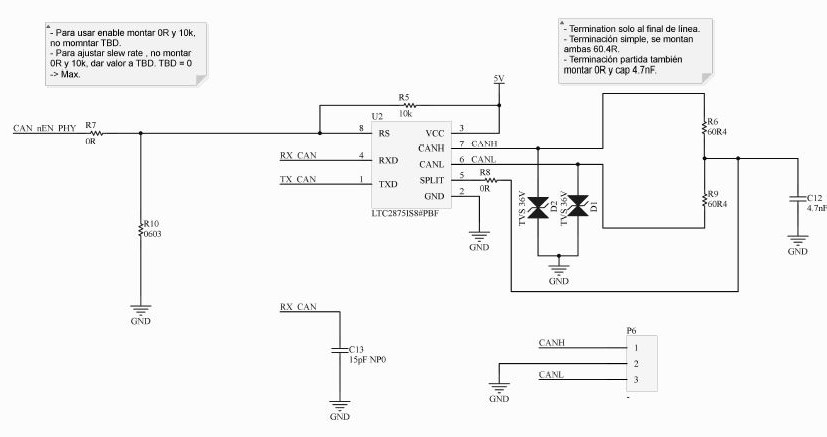
\includegraphics[scale=.75]{./Figures/sch_can.JPG}
	\caption{Esquemático de Interfaz CAN.}
	\label{fig:esquematico_can}
\end{figure}

Finalizados los subcircuitos esquemáticos, se continuó con el desarrollo del PCB. Primero, se determinaron las dimensiones de la plaqueta, manteniendo las restricciones impuestas y asegurando una cómoda posición de todos los componentes para permitir un ensamble manual. Se eligió una dimensión final de plaqueta de 100 x 80 mm. 

En el diseño del \textit{PCB} se buscó que:
\begin{itemize}
	\item Los subcircuitos quedaran separados.
	\item Los conectores se colocaran en los extremos de la plaqueta.
	\item Se respetara la aislación eléctrica de las entradas y salidas con el circuito de control.
	\item Se minimizara la longitud de las líneas de CAN y se maximizara su simetría.
\end{itemize}

La figura \ref{fig:render_pcb} muestra el render 3D del \textit{PCB} obtenido. En la parte superior se encuentran los circuitos de entradas y salidas industriales eléctricamente aislados por los optoacopladores y separados del resto del circuito. En la esquina inferior izquierda se encuentra el regulador de tensión de 5 V. En el centro el microcontrolador y a la derecha los circuitos de CAN y de USB.

\begin{figure}[htbp]
	\centering
	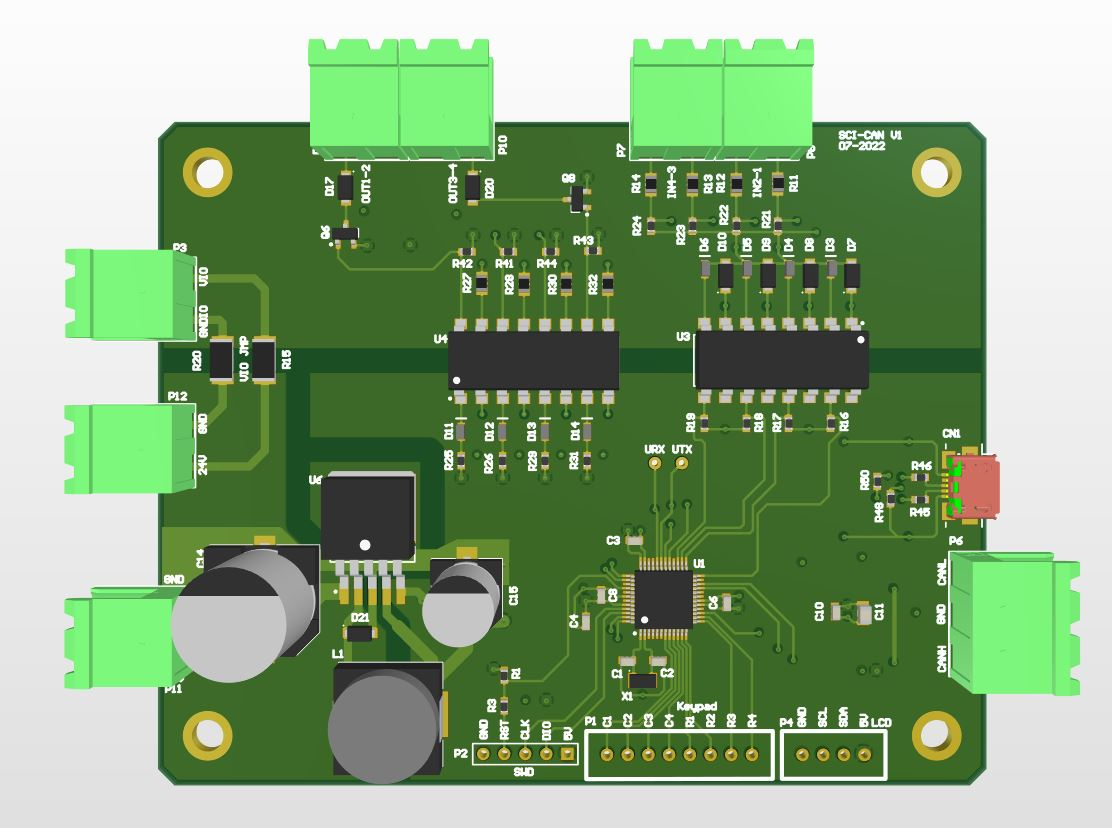
\includegraphics[scale=.4]{./Figures/pcb_sch.JPG}
	\caption{Render del \textit{PCB}.}
	\label{fig:render_pcb}
\end{figure}

\section{Desarrollo de gabinete}

Para el desarrollo del gabinete se utilizó el software de diseño mecánico Autodesk Inventor \citep{web_inventor}. Se decidió armar un ensamble que incluya todos los componentes y que sea posible su impresión 3D.

Para los componentes adquiridos, como la pantalla LCD y la matriz de botones, se tomaron los modelos 3D de uso libre de la plataforma GrabCAD \citep{web_grabcad}. Estos se verificaron para asegurarse que sus medidas correspondieran con el dispositivo físico adquirido. El modelo de la plaqueta electrónica SCI-CAN desarrollada se exportó desde el software Altium.

Una vez obtenidos los modelos de estos componentes, se realizó el desarrollo de las distintas piezas que conforman el gabinete. Como consideraciones de diseño se plantearon:

\begin{itemize}
	\item Facilitar el acceso a los conectores de la plaqueta SCI-CAN.
	\item Proteger los circuitos internos de la plaqueta SCI-CAN.
	\item Presentar el teclado y el display de forma contigua.
	\item Esconder dentro del gabinete las conexiones entre el display y el teclado con la plaqueta SCI-CAN.
	\item Minimizar la cantidad de partes y de ajustes necesarios.
	\item Limitar los ajustes a roscas métricas.
\end{itemize}

Como restricción adicional de diseño se debió mantener las dimensiones máximas de las piezas a medidas menores que la capacidad de fabricación de la impresora 3D \textit{Creality Ender-3} \citep{web_ender3}. Esto corresponde a 220 x 220 x 250 mm.

En la figura \ref{fig:ensamble} se presenta una imagen del ensamble desarrollado tomada de Inventor. Es importante notar que las piezas superiores, donde están la pantalla y el teclado, se muestran transparentes para facilitar la visualización. El ensamble consta de 3 componentes: una tapa delantera donde apoyan el display y el teclado, una caja intermedia que encierra a estos y una caja trasera donde se coloca la plaqueta de control.

\begin{figure}[h!]
	\centering
	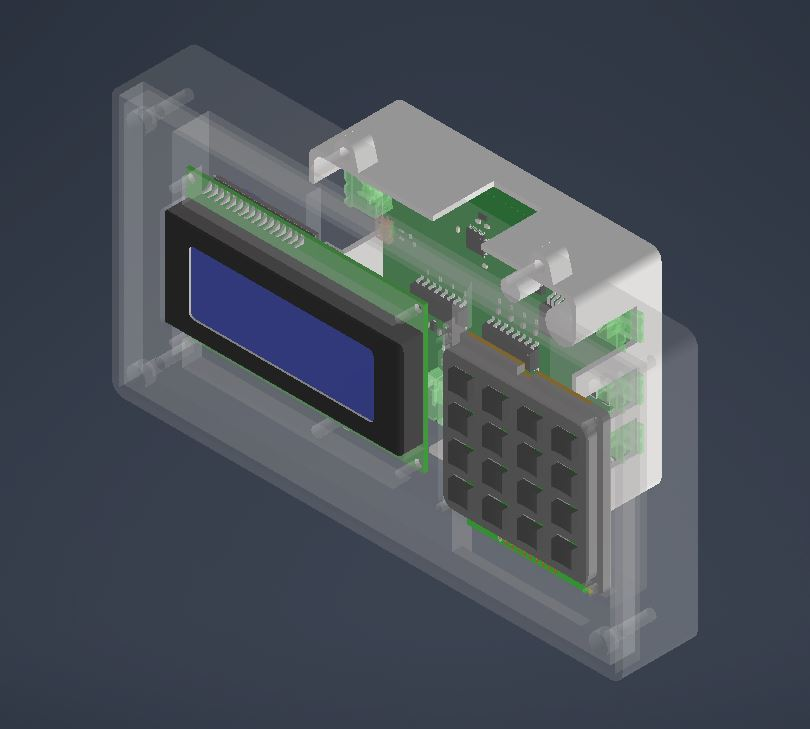
\includegraphics[scale=.6]{./Figures/asm_3d.JPG}
	\caption{Ensamble 3D de gabinete.}
	\label{fig:ensamble}
\end{figure}

\newpage

En la fabricación del conjunto se empleó el programa UltiMaker Cura \citep{web_cura3d} donde se generaron los archivos de fabricación para impresión 3D. Se decidió utilizar como material PLA, que es uno de los plásticos más económicos y simples de manipular y que cuenta con las características mecánicas apropiadas para la aplicación.